\chapter{La Configuration Du Serveur Web (Apache) Et La Sécurisation de ce dernier}

\begin{figure}[h]
    \begin{center}
 
\includegraphics[width=0.4\textwidth]{PhotoMemoire/Xampp.png}
 \caption{Logo De Xampp \cite{18}}
    \end{center}
\end{figure}
Pour La configuration J'ai utiliser le programme XAMPP qui  est un ensemble de logiciels libres qui permet de mettre en place un serveur web local sur votre ordinateur pour tester et développer des applications web. Le nom XAMPP est un acronyme qui représente les logiciels inclus dans l'ensemble :
\begin{enumerate}
	\item  X : toutes les plateformes (Windows, Linux, Mac OS X).
	\item  Apache : serveur HTTP open source.
	\item  MySQL : système de gestion de base de données relationnelle.
	\item  PHP : langage de script côté serveur pour les applications web.
	\item  Perl : langage de script polyvalent.
\begin{figure}[h]
	\begin{center}
			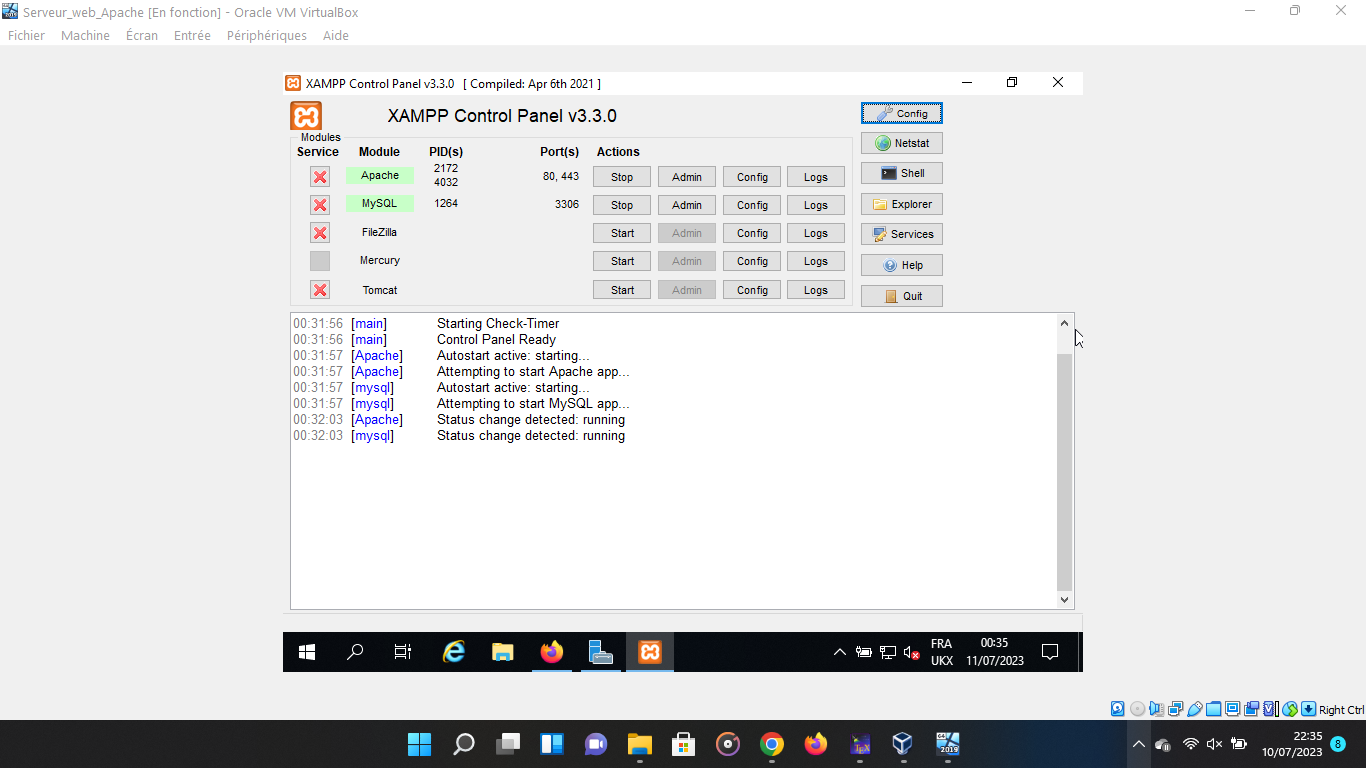
\includegraphics[width=0.7\textwidth]{ PhotoMemoire/Contro Panel.png}
			\caption{Panneau de Configuration et D'administration de Xampp}
	\end{center}
	\end{figure}
\end{enumerate}
XAMPP fournit également des fonctionnalités telles que le support SSL, le support de PHPMyAdmin pour la gestion de bases de données MySQL, et d'autres outils utiles pour le développement et le test d'applications web.\\

L'un des avantages de XAMPP est sa facilité d'utilisation, ce qui le rend particulièrement utile pour les développeurs débutants. XAMPP est disponible gratuitement en téléchargement sur le site Web d'Apache Friends, l'organisation qui développe et maintient XAMPP.


\begin{figure}[h]
	\subsection{Presentaion de Pfsense}
	 \begin{center}
	  	
\includegraphics[width=0.5\textwidth]{PhotoMemoire/pfsense.png}
	  \caption{Logo De Pfsense \cite{18}}
	 \end{center}
	 pfSense est un système d'exploitation open source basé sur FreeBSD qui est utilisé pour construire des routeurs et des pare-feux. Il est conçu pour être facile à installer, à configurer et à administrer, même pour les personnes qui n'ont pas beaucoup d'expérience dans ce domaine.\\
	 
	 pfSense est largement utilisé dans les entreprises, les établissements scolaires, les organisations gouvernementales et les fournisseurs de services Internet pour fournir une connectivité réseau sécurisée et fiable. Il offre des fonctionnalités avancées telles que la gestion de la bande passante, la surveillance de l'utilisation du réseau, le filtrage du trafic, la prise en charge du VPN, la redondance des liens WAN, la haute disponibilité, et bien plus encore.\\
	 
	 Une des caractéristiques de pfSense est la disponibilité d'un système de plug-ins et de packages tiers qui permettent d'ajouter des fonctionnalités supplémentaires au système. Il existe une grande variété de packages disponibles, allant de la surveillance de la sécurité à la gestion des réseaux sans fil.\\
	 
	 pfSense est utilisé par un grand nombre d'utilisateurs à travers le monde, et est considéré comme l'un des meilleurs systèmes d'exploitation pour les routeurs et les pare-feux. Il est également disponible gratuitement en téléchargement sur le site Web pfSense.org.\\
	 
\end{figure}

\begin{figure}[h]
	\section{Configuration de Pfsense(Snorts)}
	
	\begin{center}
		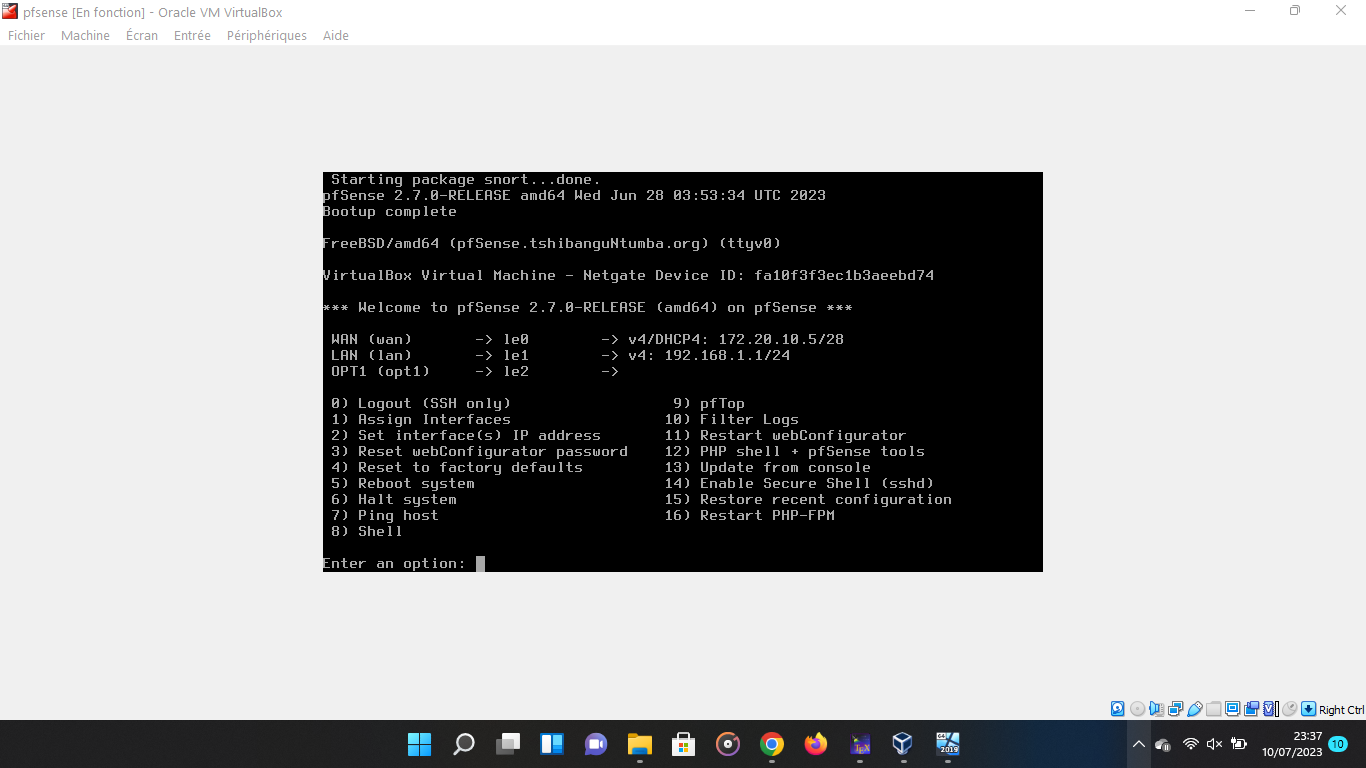
\includegraphics[width=0.8\textwidth]{ PhotoMemoire/interfacepfsense.png}
		\caption{Interface De Pfsense }
	\end{center}
	Sur cette Illustration nous voyons bien que pfsense a deux interface celle qui lui est propre et celle du serveur qu'il protege .
\end{figure}


	  \begin{figure}[h]
	  	\subsection{Configuration du Snort Pfsense} 
	  	\begin{center}
	  		
	  	 	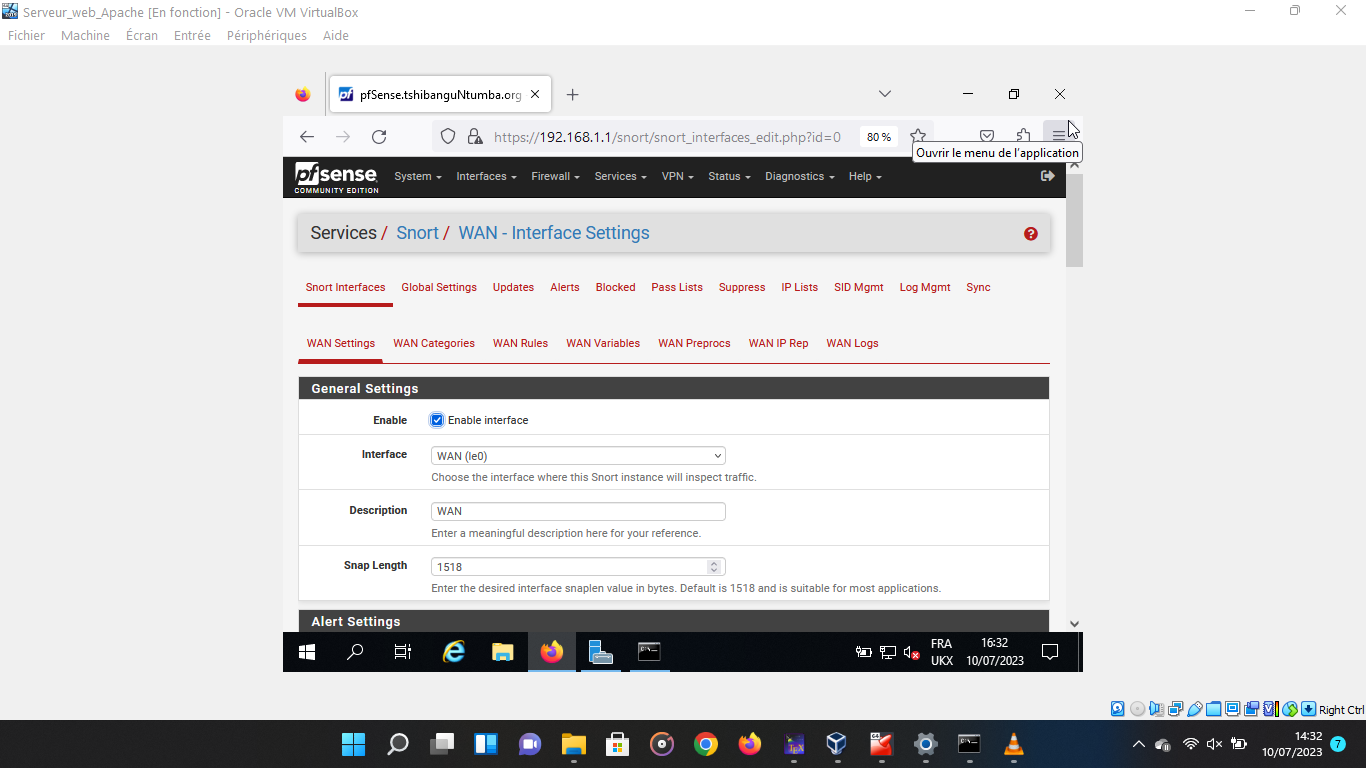
\includegraphics[width=0.8\textwidth]{photo_memoireConfig/configurationInterfaceServeur.png}
	  	 \caption{Interface Web Pfsense }
	  	\end{center}
	 \end{figure}
	 
	 \begin{figure}[h]
	  \begin{center}
	   	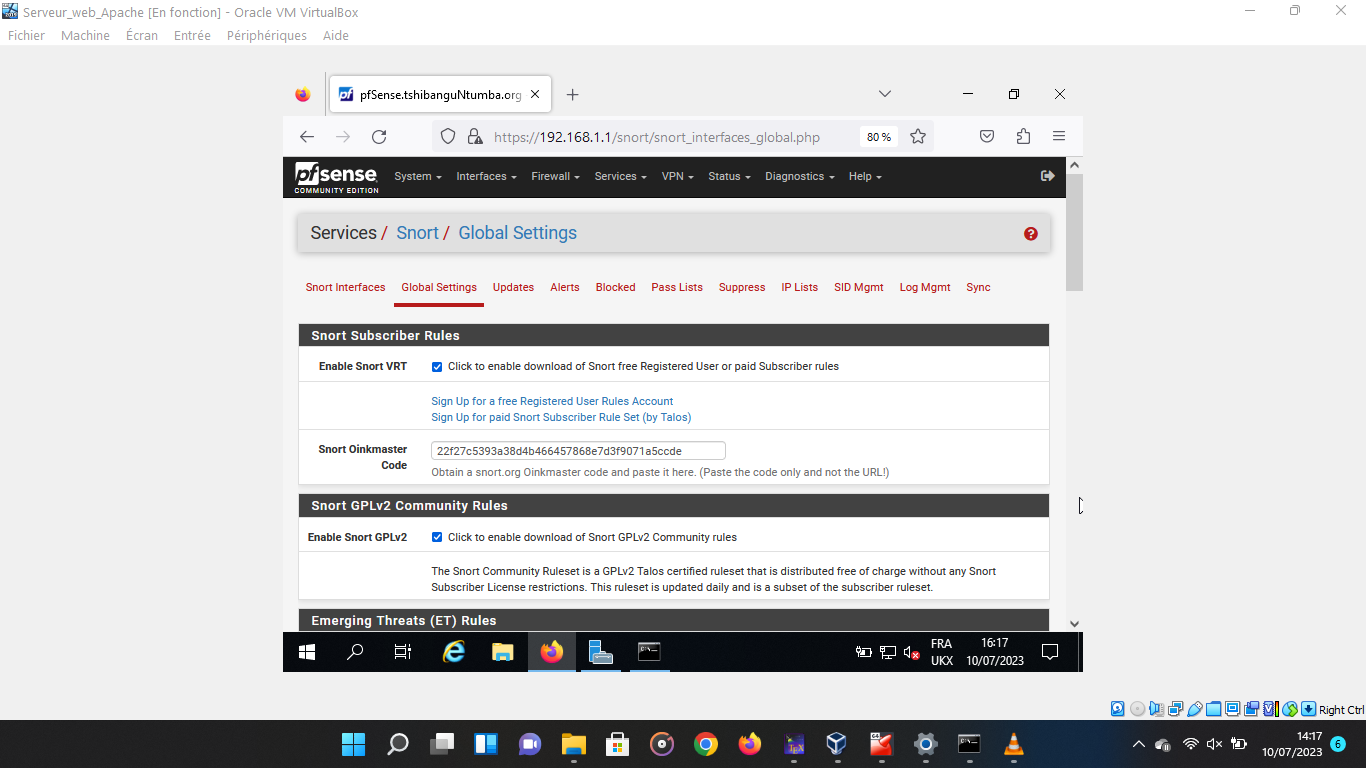
\includegraphics[width=0.8\textwidth]{photo_memoireConfig/Global_settings.png}
	   \caption{Configuration des paramètres Globaux de l'interface}
	    \end{center}
	 \end{figure}
	 
	 \begin{figure}[h]
	 	  \begin{center}
	 	 	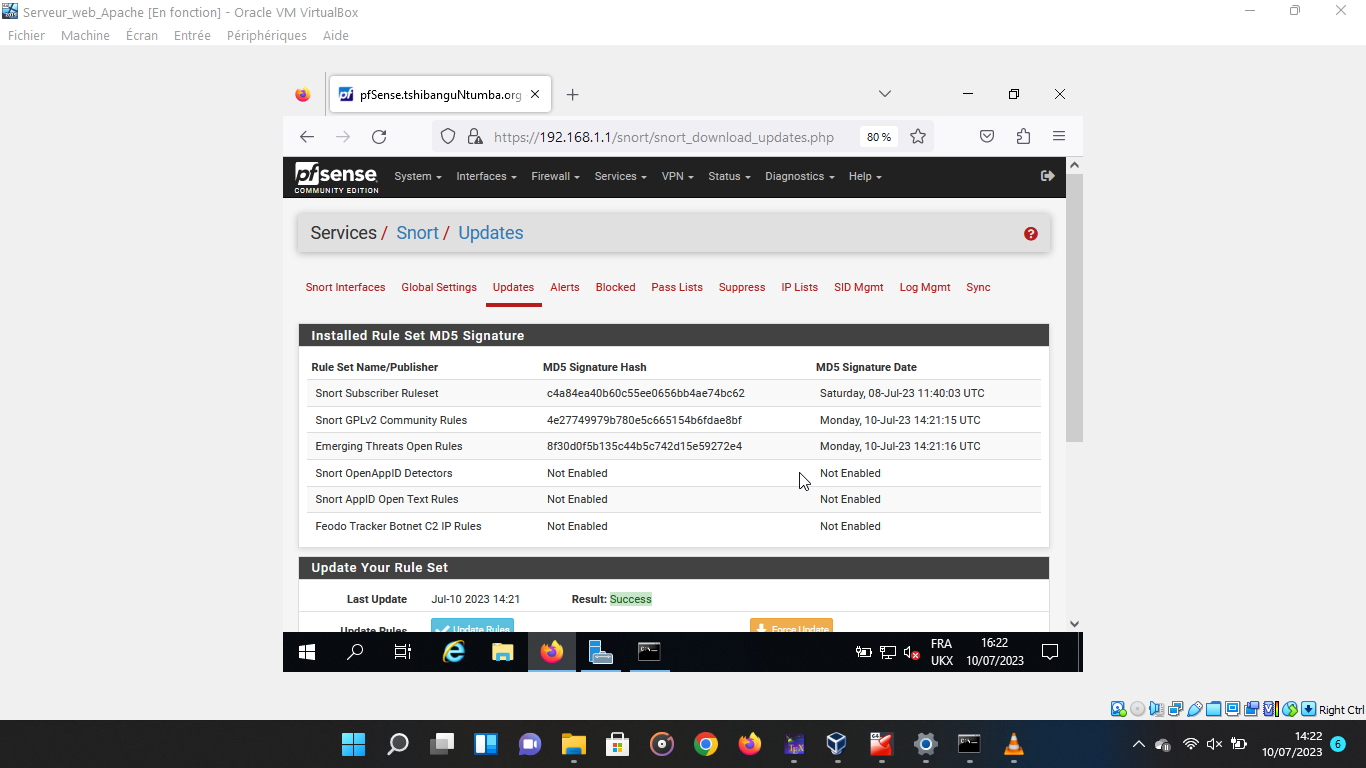
\includegraphics[width=0.8\textwidth]{photo_memoireConfig/Update_des Cles MD5.png}
	 	 \caption{Mise  a jour des clés de chiffrements MD5, Et des Règles de Filtrage }
	\end{center}
	 \end{figure}
 


\begin{figure}[h]
	\section{Capture Des Test}
	\paragraph{}
	Ici nous voyons clairement que le Snort a Bel et bien intercepter l'adresse IP
	De l'attaquant  et alerte L'interface Web d'une tentative d'intrusion.
 \begin{center}
			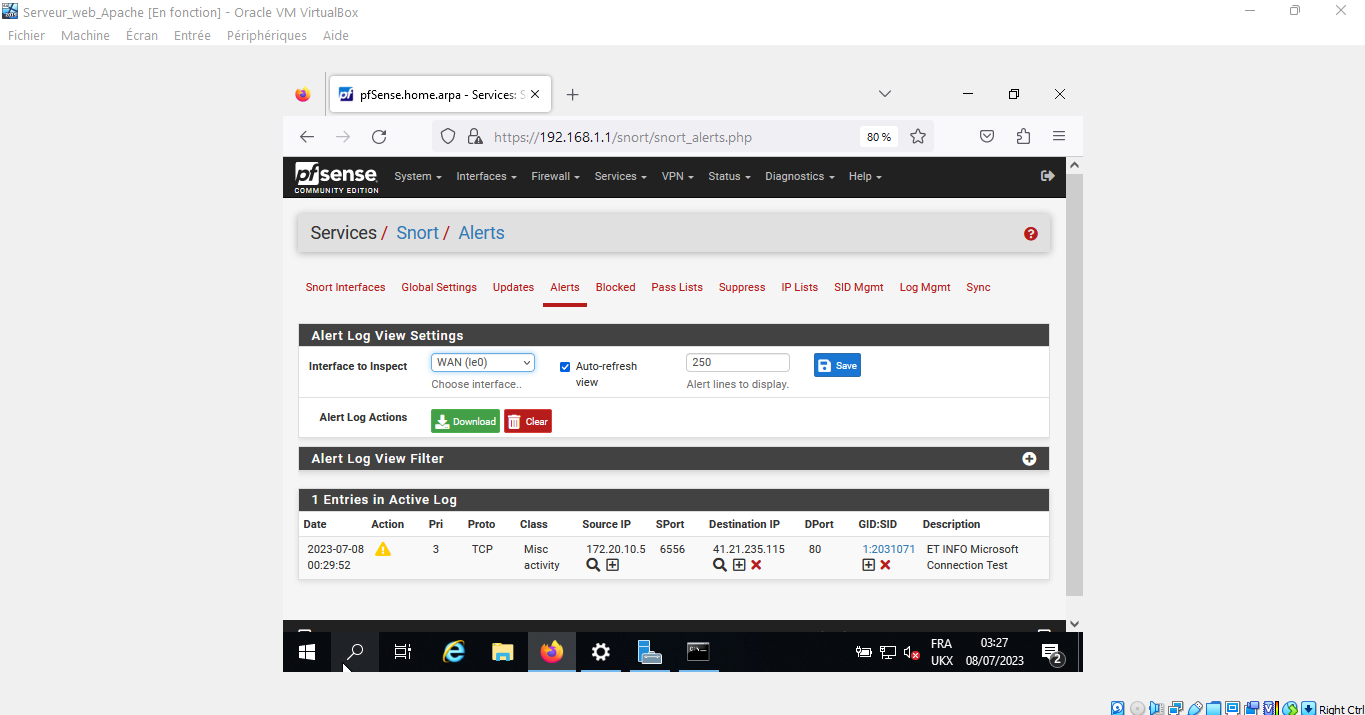
\includegraphics[width=0.8\textwidth]{photo_memoireConfig/Alert_ip.png}
		\caption{Alerte D'intrusion Pfsense}
	\end{center}
\end{figure}
 
\begin{figure}[h]
	\paragraph{}
	Sur cette Illustration on voit que le Snort a bloquer l'adresse de l'attaquant et l'a interdit d'accès.
	 \begin{center}
		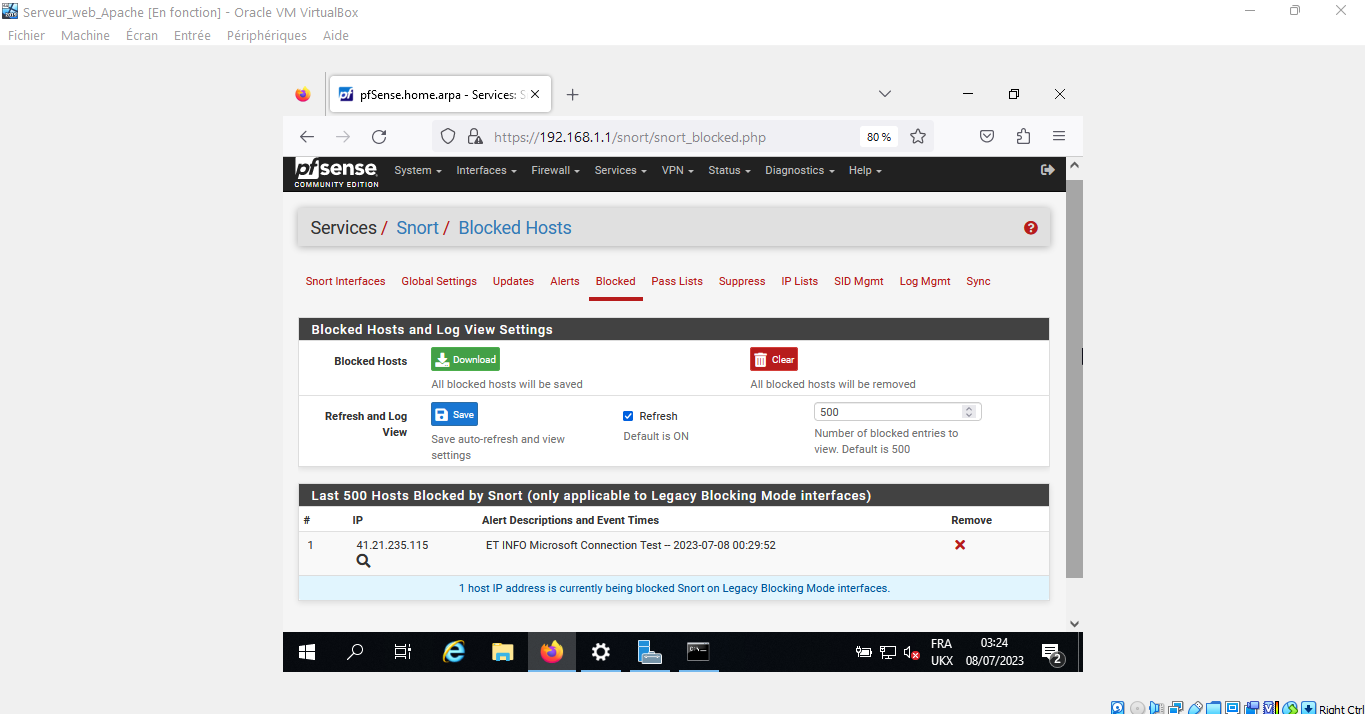
\includegraphics[width=0.8\textwidth]{photo_memoireConfig/Blocked_IP.png}
		\caption{Adresse Ip Isolées}
 \end{center}
\end{figure}
 
\begin{figure}[h]
	\section{Environnement de Test}
	\subsection{Virtual Box}
	\begin{center}
		
\includegraphics[width=0.8\textwidth]{PhotoMemoire/Virtualbox.png}
		\caption{ Le logo Virutal Box }\cite{18}
	\end{center}
	Oracle VirtualBox est un logiciel de virtualisation open source qui permet de créer des machines virtuelles sur votre ordinateur. Les machines virtuelles sont des environnements virtuels qui peuvent exécuter différents systèmes d'exploitation, tels que Windows, Linux, MacOS et bien d'autres, à l'intérieur d'un hôte (votre ordinateur).\\
	
	VirtualBox est utilisé pour de nombreuses tâches, notamment pour tester des applications, pour développer des logiciels, pour créer des environnements de test, pour exécuter des systèmes d'exploitation différents, pour configurer des serveurs en environnement isolé, etc.\\
	
	VirtualBox fonctionne en émulant des composants matériels tels que le processeur, la mémoire, le stockage et les interfaces réseau. Il fournit également des fonctionnalités avancées telles que le partage de fichiers entre l'hôte et la machine virtuelle, la prise en charge de l'USB, la virtualisation des cartes graphiques, la prise en charge de plusieurs écrans, et bien plus encore.\\
	
	VirtualBox est développé et maintenu par Oracle Corporation et est disponible en téléchargement gratuit sur son site Web. Il est compatible avec une grande variété de systèmes d'exploitation hôtes, notamment Windows, Linux, MacOS et Solaris.\\ 
\end{figure}

\begin{figure}[h]
	Les machines Virtuelle on permis les différents test dans ce Travail.
	 \begin{center}
	 	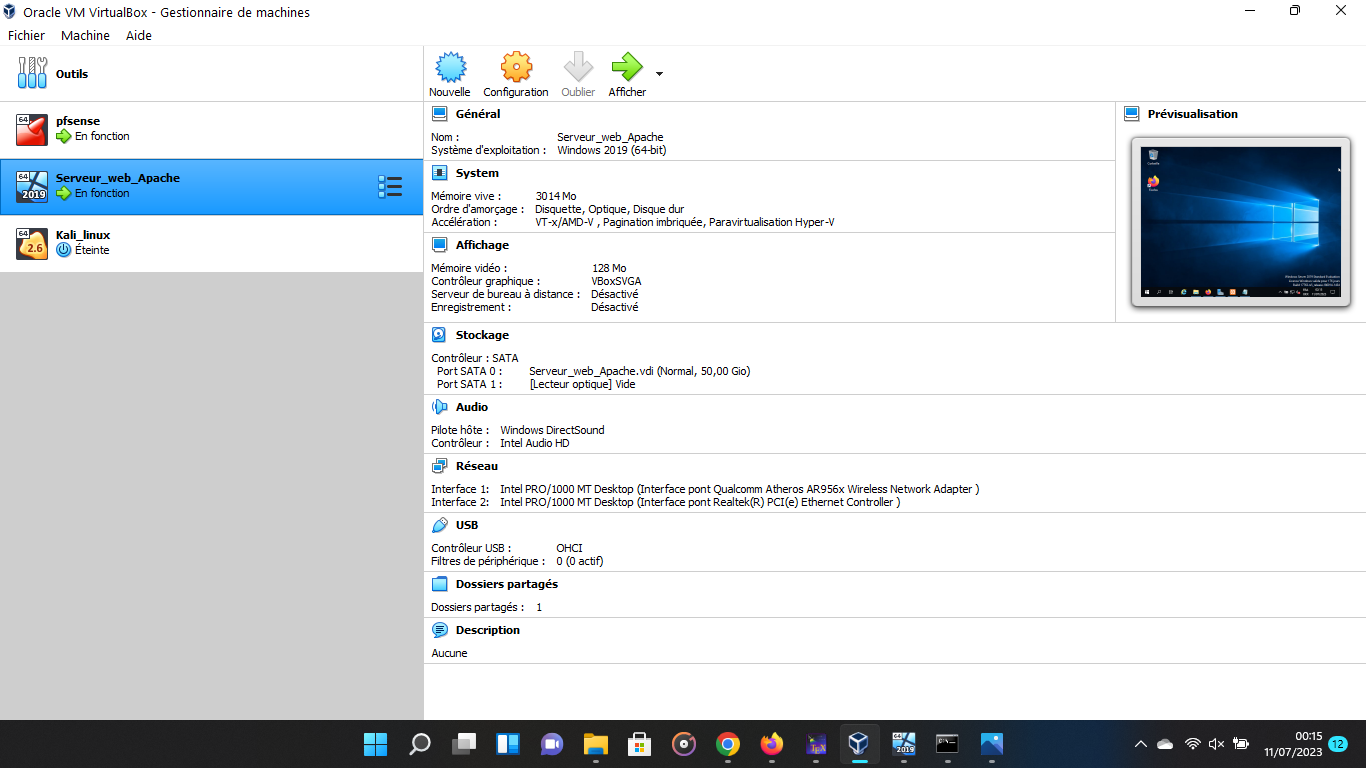
\includegraphics[width=0.8\textwidth]{PhotoMemoire/machineutilisee.png}
	 	\caption{ Les Machines Utilisées Pour les Test}	
	 \end{center}
\end{figure}
\begin{figure}[h]
	 Site Web Utilisé Pour Les Test
	\begin{center}
		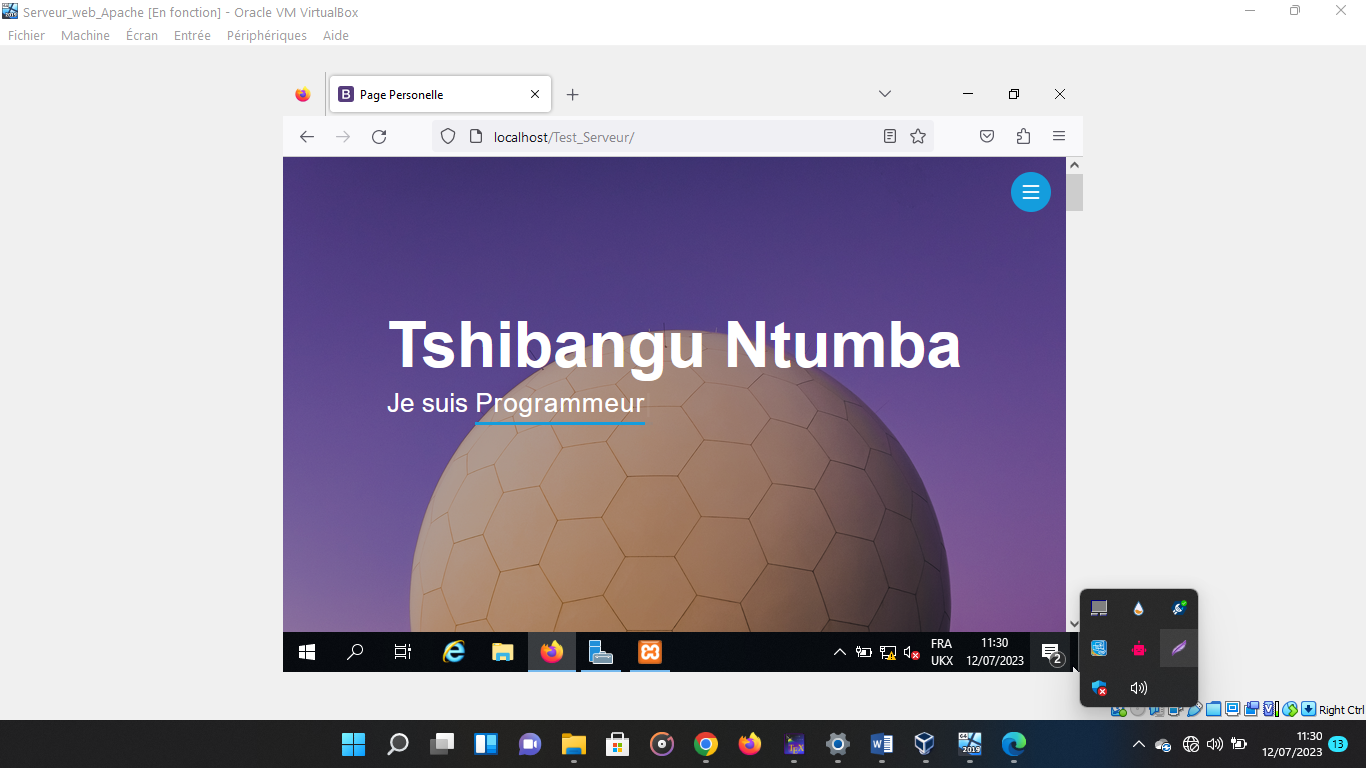
\includegraphics[width=0.8\textwidth]{PhotoMemoire/serveur _Web.png}
		\caption{ Site Web Utilisé Pour les Test}
	\end{center}
\end{figure}



